% This is LLNCS.DEM the demonstration file of
% the LaTeX macro package from Springer-Verlag
% for Lecture Notes in Computer Science,
% version 2.4 for LaTeX2e as of 16. April 2010
%
\documentclass{llncs}
%
\usepackage{makeidx}  % allows for indexgeneration
\usepackage{graphicx}
%
\begin{document}
%
%
\mainmatter              % start of the contributions
%
\title{OpenML: A Collaborative Science Platform}
%
\titlerunning{OpenML: A Collaborative Science Platform}  
%
\author{Jan N. van Rijn\inst{1} \and Bernd Bischl\inst{2} \and Luis Torgo\inst{3} \and Bo Gao\inst{4} \and Venkatesh Umaashankar\inst{5} \and Simon Fischer\inst{5} \and Patrick Winter\inst{6} \and Bernd Wiswedel\inst{6} \and Michael R. Berthold\inst{7} \and Joaquin Vanschoren\inst{1}}
%
\authorrunning{van Rijn et al.} % abbreviated author list (for running head)
%
%%%% list of authors for the TOC (use if author list has to be modified)
\tocauthor{Jan N. van Rijn, Bernd Bischl, Luis Torgo, Bo Gao, Venkatesh Umaashankar, Simon Fischer, Patrick Winter, Bernd Wiswedel, Michael R. Berthold, Joaquin Vanschoren}
%

\institute{
Leiden University, Leiden, Netherlands,
\email{\{jvrijn,joaquin\}@liacs.nl}
\and
TU Dortmund, Dortmund, Germany,
\email{bischl@statistik.tu-dortmund.de}
\and
University of Porto, Porto, Portugal,
\email{ltorgo@inescporto.pt}
\and
KU Leuven, Leuven, Belgium,
\email{bo.gao@cs.kuleuven.be}
\and
Rapid-I GmbH, Dortmund, Germany,
\email{\{venkatesh,fischer\}@rapid-i.com}
\and
KNIME.com AG,
\email{\{patrick.winter,Bernd.Wiswedel\}@knime.com}
\and
University of Konstanz, Konstanz, Germany,
\email{Michael.Berthold@uni-konstanz.de}
}

\maketitle              % typeset the title of the contribution

\begin{abstract}

We present OpenML, a novel open science platform that provides easy access to machine learning data, software and results to encourage further study and application. It organizes all submitted results online so they can be easily found and reused, and features a web API which is being integrated in popular machine learning tools such as Weka, KNIME, RapidMiner and R packages, so that experiments can be shared easily.

\keywords{Experimental Methodology, Machine Learning, Databases, Meta-Learning}

\end{abstract}

\section{Introduction}

Research in machine learning and data mining can be speeded up tremendously by moving empirical research results ``out of people's heads and labs, onto the network and into tools that help us structure and alter the information''~\cite{Nielsen2008}. The massive streams of experiments that are being executed to benchmark new algorithms, test hypotheses or model new datasets have many more uses beyond their original intent, but are often discarded or their details are lost over time. In this paper, we present OpenML\footnote{OpenML can be found at \texttt{http://www.openml.org}.}, an open science platform for machine learning research. OpenML is a website where researchers can share their datasets, implementations and experiments in such a way that they can easily be found and reused by others. It offers a web API through which new resources and results can be submitted, and is being integrated in a number of popular machine learning and data mining platforms, such as Weka, RapidMiner, KNIME, and data mining packages in R, so that new results can be submitted automatically. Vice versa, it enables researchers to easily search for certain results (e.g., evaluations on a certain dataset), to directly compare certain techniques against each other, and to use all submitted data in advanced queries. An overview of the key components of OpenML is provided in Figure~\ref{fig:openmlOverview}.

\begin{figure}

 \centering

 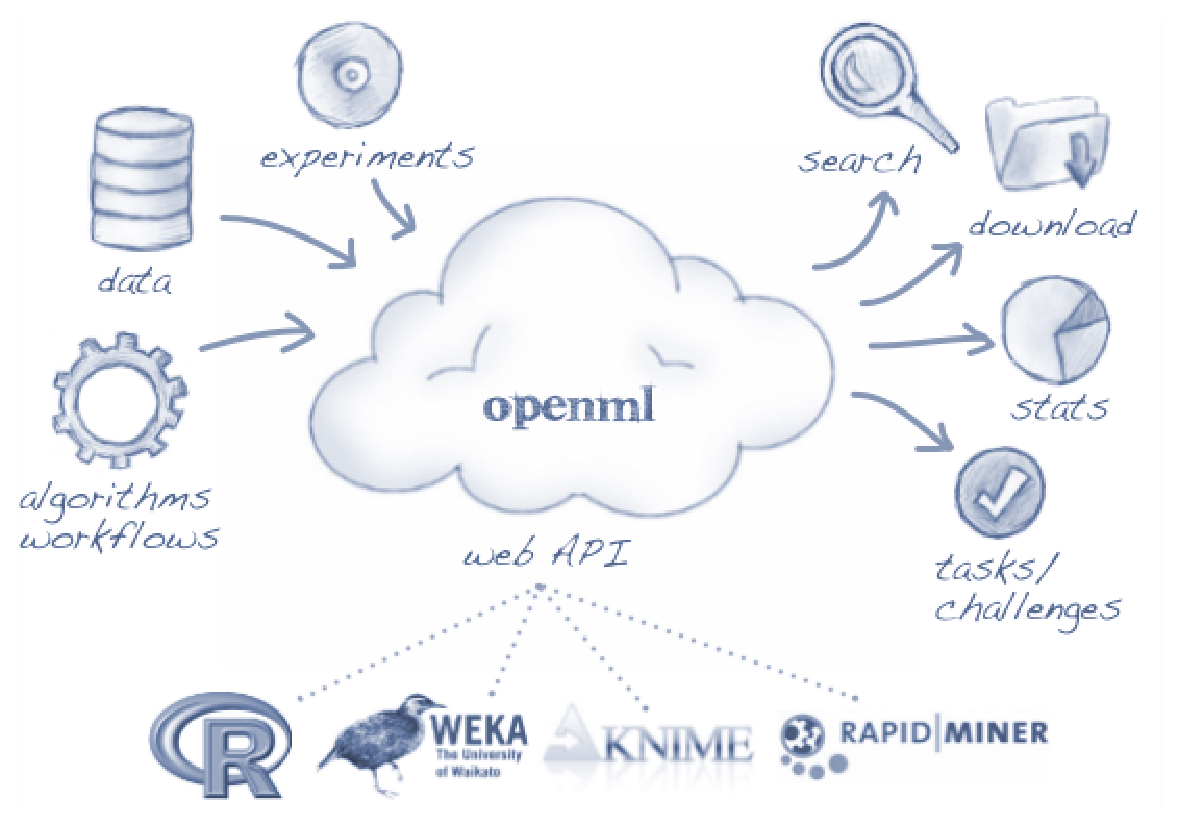
\includegraphics[scale=0.35]{openmldiagram.eps}

 \label{fig:openmlOverview}

 \caption{Components of the OpenML platform}

\end{figure}

OpenML engenders a novel, collaborative approach to experimentation with important benefits. First, many questions about machine learning algorithms won't require the laborious setup of new experiments: they can be answered on the fly by querying the combined results of thousands of studies on all available datasets. OpenML also keeps track of experimentation details, ensuring that we can easily reproduce experiments later on, and confidently build upon earlier work~\cite{Hirsh2008}. Reusing experiments also allows us to run large-scale machine learning studies, yielding more generalizable results~\cite{Hand2006} with less effort. Finally, beyond the traditional publication of algorithms in journals, often in a highly summarized form, OpenML allows researchers to share all code and results that are possibly of interest to others, which may boost their visibility, speed up further research and applications, and engender new collaborations.

\section{Sharing Experiments}

To make experiments from different researchers comparable, OpenML uses \emph{tasks}, well-described problems to be solved by a machine learning algorithm or workflow. A typical task would be: \emph{Predict (target) attribute X of dataset Y with maximal predictive accuracy}. Somewhat similar to a data mining challenge, researchers are thus challenged to build algorithms that solve these tasks.
Different tasks can be defined, e.g., parameter optimization, feature selection and clustering. They can be searched online, and will be automatically generated for newly submitted datasets.
OpenML provides all necessary information to complete the task, such as a URL to download the input dataset, and what information should be submitted to the server. For some tasks, e.g., predictive tasks, it offers more structured input and output, such as exact train and test splits for cross-validation, and a submission format for all predictions. The server will then evaluate the predictions and store the scores for various evaluation metrics.

An attempt to solve a task is called a \emph{run}, and includes the task itself, the algorithm or workflow (i.e., implementation) used, and a file detailing the obtained results. These are all submitted to the server, where new implementations will be registered. Workflows are represented as a set of algorithms, and can be downloaded into the workbenches for detailed inspection. For each implementation, an overview page will be generated containing data about all tasks on which this algorithm was run. This will detail the performance of the algorithm over a potentially wide range of datasets, with various parameter settings. For each dataset, a similar page is created, containing a ranking of algorithms that were run on tasks with that dataset as input.

OpenML provides a RESTful API for downloading tasks and uploading datasets, implementations and results. This API is currently being integrated in various machine learning platforms such as Weka, R packages, RapidMiner and KNIME. For instance, in WEKA\footnote{A beta version can be downloaded from the OpenML website.}, OpenML is integrated as part of the Weka Experimenter. Given a task, it automatically downloads all associated input data, runs the experiment, and uploads the results to OpenML.

\section{Searching OpenML}

OpenML links various bits of information together in a single database. All results for different algorithms on the same tasks are stored in such a way that algorithms can directly be compared against each other (using various evaluation measures), and parameter settings are stored so that the impact of individual parameters can be tracked.
Moreover, for all datasets, it calculates meta-data concerning their features (e.g., type, distinct values or mean and standard deviation) and their distributions, such as the number of features, instances, missing values, default accuracy, class entropy and landmarking results~\cite{Peng2002}. Likewise, for algorithms, it includes information about the (hyper)parameters and properties, such as whether the algorithm can handle nominal/numeric features, whether it can perform classification and/or regression and a bias-variance profile.

OpenML allows users to easily search for results of interest. First, it stores textual descriptions for datasets, algorithms and implementations so that they can be found through simple keyword searches, linked to overview pages that detail all related results. Second, runs can be searched to directly compare many algorithms over many datasets (e.g., for benchmarking). Furthermore, the database can be queried directly through an SQL editor, or through pre-defined advanced queries such as ``Show the effect of a parameter P on algorithm A on dataset D'' and ``Draw the learning curve for algorithm A on dataset D''.\footnote{See the `Advanced' tab on \texttt{http://www.openml.org/search}.} The results of such queries are displayed as data tables, scatterplots or line plots, which can be downloaded directly.

\section{Related Work}

OpenML builds on previous work on \emph{experiment databases}~\cite{Vanschoren2012}, but also enhances it by markedly facilitating the sharing of new experiments through the web API and by making results much easier to find and compare.

In terms of sharing algorithms or workflows, it is somewhat similar to MyExperiment\footnote{\texttt{http://www.myexperiment.org/}}, an online repository where users can search and share workflows so that interesting workflows can be reused. However, MyExperiment offers little support for storing the \emph{results} of workflows, or comparing workflows based on performance metrics.

On the other hand, MLComp\footnote{\texttt{http://www.mlcomp.org/}} is a platform on which  users can run their algorithms on known datasets (or vice versa). These runs are performed on the servers of MLComp, which saves the user resources. Although very useful, especially for comparing runtimes, OpenML differs from MLComp in two key aspects: First, OpenML allows users much more flexibility in running experiments: new tasks can easily be introduced for novel types of experiments and experiments can be run in any environment. It is also being integrated in data mining platforms that researchers already use in daily research. Finally, OpenML allows more advanced search and query capabilities that allow researchers to reuse results in many ways beyond direct comparisons, such as meta-learning studies~\cite{Vanschoren2012}.

\section{Conclusions and Future Work}
OpenML aims to engender an open, collaborative approach to machine learning research. Experiments can be shared in full detail, which generates a large amount of reproducible results available for everyone. Moreover, integration with popular data mining tools will make it very easy for researchers to share experiments with OpenML and the community at large.

Future work includes support for a broader range of task types, e.g., time series analyses, graph mining and text mining.

\subsubsection*{Acknowledgments}

This work is supported by grant 600.065.120.12N150 from the Dutch Fund for Scientific Research (NWO), and by the IST Programme of the European Community, under the Harvest Programme of the PASCAL2 Network of Excellence, IST-2007-216886.

\bibliography{pkdd2013}
\bibliographystyle{splncs03}

%
% second contribution with nearly identical text,
% slightly changed contribution head (all entries
% appear as defaults), and modified bibliography
%
\end{document}
